\documentclass{article}

\usepackage[french]{babel} 
\usepackage[T1]{fontenc}
\usepackage{lmodern}
\usepackage[utf8]{inputenc}

\usepackage{float}
\usepackage{mathtools}
\DeclarePairedDelimiter{\ceil}{\lceil}{\rceil}
\usepackage{fancyhdr}
\usepackage{extramarks}
\usepackage{amsmath}
\usepackage{amsthm}
\usepackage{amsfonts}
\usepackage{amssymb}
\usepackage{tikz}
\usepackage{graphicx}
\usepackage{pdfpages}
\usepackage[makeroom]{cancel}
\usepackage{karnaugh-map}

%
% Basic Document Settings
%

\topmargin=-0.45in
\evensidemargin=0in
\oddsidemargin=0in
\textwidth=6.5in
\textheight=9.0in
\headsep=0.25in

\linespread{1.1}

\pagestyle{fancy}

%
% Create Problem Sections
%

\newcommand{\enterProblemHeader}[1]{
    \nobreak\extramarks{}{Question \arabic{#1} continued on next page\ldots}\nobreak{}
    \nobreak\extramarks{Question \arabic{#1} (suite)}{Suite de la question \arabic{#1} à la page suivante\ldots}\nobreak{}
}

\newcommand{\exitProblemHeader}[1]{
    \nobreak\extramarks{Question \arabic{#1} (suite)}{Suite de la question \arabic{#1} à la page suivante\ldots}\nobreak{}
    \stepcounter{#1}
    \nobreak\extramarks{Question \arabic{#1}}{}\nobreak{}
}

\setcounter{secnumdepth}{0}
\newcounter{partCounter}
\newcounter{homeworkProblemCounter}
\setcounter{homeworkProblemCounter}{1}
\nobreak\extramarks{Question \arabic{homeworkProblemCounter}}{}\nobreak{}

%
% Homework Problem Environment
%
% This environment takes an optional argument. When given, it will adjust the
% problem counter. This is useful for when the problems given for your
% assignment aren't sequential. See the last 3 problems of this template for an
% example.
%
\newenvironment{homeworkProblem}[1][-1]{
    \ifnum#1>0
        \setcounter{homeworkProblemCounter}{#1}
    \fi
    \section{Tâche \arabic{homeworkProblemCounter}}
    \setcounter{partCounter}{1}
    \enterProblemHeader{homeworkProblemCounter}
}{
    \exitProblemHeader{homeworkProblemCounter}
}

%
% Homework Details
%   - Title
%   - Due date
%   - Class
%   - Section/Time
%   - Instructor
%   - Author
%

\newcommand{\hmwkTitle}{Travail\ pratique\ 4}
\newcommand{\hmwkDueDate}{8 Décembre 2023}
\newcommand{\hmwkClass}{\ \ IFT 3913}
\newcommand{\hmwkClassTime}{}%Section 
\newcommand{\hmwkClassInstructor}{Professeur: Michalis Famelis}
\newcommand{\hmwkAuthorName}{\textbf{Killian Gervais \& Gabriel Hazan}}

%
% Title Page
%

\title{
    \vspace{2in}
    \textmd{\textbf{\hmwkClass:\ \hmwkTitle}}\\
    \normalsize\vspace{0.1in}\small{Pour\ le\ \hmwkDueDate\ à 23:59 }\\
    \vspace{0.1in}\large{\textit{\hmwkClassInstructor\ \hmwkClassTime}}
    \vspace{3in}
}

\author{\hmwkAuthorName}
\date{}

\renewcommand{\part}[1]{\textbf{\large Partie \Alph{partCounter}}\stepcounter{partCounter}\\}

% Probability commands: Expectation, Variance, Covariance, Bias
\newcommand{\E}{\mathrm{E}}
\newcommand{\Var}{\mathrm{Var}}
\newcommand{\Cov}{\mathrm{Cov}}
\newcommand{\Bias}{\mathrm{Bias}}

\tikzstyle{bag} = [align=center]
\begin{document}

\maketitle
\thispagestyle{empty}

\pagebreak
% Tache 1
\begin{homeworkProblem}
    D'après la spécification donnée, on a deux types d'entrées: les devises (\textit{currencies}) et les montants (\textit{amounts}). Soit les devises du programme $P_C$ défini sur \{USD, CAD, GBP, EUR, CHF, AUD\} avec \\$C$ = Currencies = \{USD, CAD, GBP, EUR, CHF, AUD, JPY, INR, NZD\}, cette dernière pourrait être agrandie au besoin, et les montants du programme $P_A$ défini sur [0, 1 000 000], l'intervalle des valeurs valides, avec $A$ = Amounts = Réels.\\
    \linebreak
    Il y a deux classes d'équivalences pour les devises:
    \begin{itemize}
        \item[$\bullet$] Les valeurs d'entrées valides:\quad $C_1 = P_C =$ \{USD, CAD, GBP, EUR, CHF, AUD\}
        \item[$\bullet$] Les valeurs d'entrées invalides:\quad $C_2 =$ \{JPY, IRN, NZD\}
    \end{itemize}
    On choisit une valeur de chaque classe, pour pouvoir tester le cas ou l'une des devises est valide tandis que l'autre ne l'est pas, ainsi qu'une seconde valeur de devise valide pour tester les conversion de montant pour créer notre jeu de test $T_C$ = \{USD, EUR, JPY\}.\\
    \linebreak
    Pour les montants, il y a trois classes d'équivalences, $a \in \mathbb{R}$:
    \begin{itemize}
        \item[$\bullet$] Les valeurs appartenant à $P_A$:\quad $A_1 = \{0 \leq a \leq 1\ 000\ 000\}$
        \item[$\bullet$] Les valeurs invalides inférieures à $P_A$:\quad $A_2 = \{a < 0\}$
        \item[$\bullet$] Les valeurs invalides supérieure à $P_A$:\quad $A_3 = \{a > 1\ 000\ 000\}$
    \end{itemize}
    On choisit choisit une valeur "typique" dans chaque classe d'équivalence et plusieurs aux bornes de celles-ci pour créer le jeu de test $T_A = \{-2\ 222\ 222, -0.09, 0, 500\ 000, 1\ 000\ 000, 1\ 000\ 000.01, 2\ 222\ 222\}$.\\

    Si une entrée est invalide, on s'attend à ce que le code ne s'arrête pas, il est donc capable de s'adapter à une mauvaise entrée fournie par l'utilisateur, que ce soit pour une devise ou un montant. On s'attend a ce que ce soit la classe MainWindow qui gère les entrées invalides. Puisque, selon la spécifiation, le type des données retournées par ces méthodes sont des double positifs on s'attend à recevoir "-1.0" comme résulat lors d'une entrée invalide.
\end{homeworkProblem}

%Tache 2
\begin{homeworkProblem}
    On va suivre la méthode des 5 critères de sélection de jeux de tests de la méthode boîte blanche dans le but de créer nos jeux de tests, lorsque ceux-ci sont applicables.\\
    \hfill\\
    Commençons par la méthode \textit{convert} de la classe MainWindow:
    \begin{itemize}
        \item[\underline{Couverture des instructions}:]
        Puisque les boucles utilisées sont des \textit{for} il suffit que $currencies.size() > 0$ pour que les boucles soient exécutées au moins une fois, avec \textit{currencies} la liste des devises acceptées. Les structures conditionnelles sont toutes des \textit{if}, leur code est exécuté si leur condition est vraie. De plus, on note que le premier et le troisième sont dans les boucles \textit{for}. Le code du premier \textit{if} est exécuté quand \textit{currency2} est dans la liste des devises, même chose pour le code du troisième mais avec \textit{currency1} cette fois. Le code du dernier, qui est en fait le second \textit{if} de la méthode, est exécuté lorsque le code du premier l'a été, ils partagent donc la même classe du domaine. D'après cela, on obtient la classe d'équivalence suivante:\\
        $D_1$ = \{(\textit{currency1}, \textit{currency2}) | \textit{currencies.size()} > 0\ \&\ \textit{currency1}, \textit{currency2} $\in$ \textit{currencies}\}\\
        Avec celle-ci, tout le code est exécuté au moins une fois. On peut donc prendre le jeu de test: \{"US Dollar", "Euro"\}, ces deux valeurs étant définies dans la classe Currency.
        
        \pagebreak
        
        \item[\underline{Couverture des arcs du graphe de flot de contrôle}:] On obtient le graphe de flot contrôle suivant
        \begin{figure}[H]\centering
            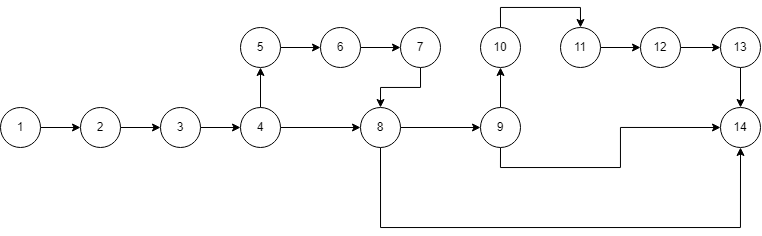
\includegraphics[width = \linewidth]{control-flow-graph-MainWindow.png}
        \end{figure}
        Les numéros correspondent à la ligne de code qui n'est pas un commentaire correspondante dans la méthode, 1 la première ligne après le bracket d'ouverture. On déjà énoncé les conditions qui font que les \textit{if} et les boucles \textit{for} sont exécutés ci-haut. On veut cependant ajouter les cas qui font que leur conditions sont fausses. D'où:\\
        $D_1$ = \{(\textit{currency1}, \textit{currency2}) | \textit{currencies.size()} > 0 \& \textit{currency1}, \textit{currency2} $\in$ \textit{currencies}\}\\
        $D_2$ = \{\textit{curr.1}, \textit{curr.2}) | \textit{currencies.size()} = 0\}\\
        $D_3$ = \{(\textit{currency1}, \textit{currency2})|\textit{currencies.size()} > 0, \textit{currency1}$\not\in$\textit{currencies} \& \textit{currency2}$\in$\textit{currencies}\}
        $D_4$ = \{(\textit{currency1}, \textit{currency2})|\textit{currencies.size()} > 0, \textit{currency1}$\in$\textit{currencies} \& \textit{currency2}$\not\in$\textit{currencies}\}\\
        \hfill\\
        Il n'y a pas le cas où les deux devises ne sont pas dans la liste, puisque si la deuxième ne l'est pas alors la partie du code qui vérifie si la première se trouve dans la liste n'est pas exécutée. On peut donc prendre le jeu de test suivant: \{\{("US Dollar", "Euro") | \textit{currencies = $\emptyset$}\}, \{("US Dollar", "Euro"), ("Australian Dollar", "US Dollar"), ("Euro", "US Dollar") | "US Dollar", "Euro" $\in$ \textit{currencies}\}\}, puisque le dollar australien n'est pas défini dans Currency tandis que les deux autres le sont.\\
        
        \item[\underline{Couverture des chemins indépendants du graphe de flot de contrôle}:] La compléxité cyclomatique est $V(G) = e-n+2 = 18 - 14 + 2 = 1 + d = 1 + 5 = 6$. On définit maintenant une base de 6 chemins indépendants du graphe de flot:
        \begin{itemize}
            \item[$\bullet$] 1-2-3-4-8-14: la liste des devises est vide, $D_1$ = \{(\textit{currency1}, \textit{currency2}) | \textit{currencies = $\emptyset$}\}
            \item[$\bullet$] 1-2-3-4-5-4-8-14: $D_2$ = \{(\textit{currency1}, \textit{currency2}) | \textit{currency2} $\not\in$ \textit{currencies}, \textit{currency1} $\in$ \textit{currencies}\}
            \item[$\bullet$] 1-2-3-4-5-6-7-8-9-10-9-14: $D_3$ = \{(\textit{curr.1}, \textit{curr.2}) | \textit{curr.2} $\in$ \textit{currencies}, \textit{curr.1} $\not\in$ \textit{currencies}\}
            \item[$\bullet$] 1-2-3-4-5-6-7-8-9-10-11-12-13-14: $D_4$ = \{(\textit{curr.1}, \textit{curr.2}) | \textit{curr.2}, \textit{curr.1} $\in$ \textit{currencies}\}
        \end{itemize}
        On a utilisé tous les arcs du graphe et il ne reste donc plus de chemins linéairement indépendants. Le jeu de test créer à l'étape précédente répondait déjà à ces critères, on le conserve donc tel quel.\\

        \item[\underline{Couverture des conditions}:] Il n'y a pas de conditions composées dans cette méthode. Ce critère n'est donc pas applicable.\\
        
        \item[\underline{Couverture des i-chemins}:] Les deux boucles sont des boucles simples. Il n'y a pas un grand intêret à faire l'ensemble des cas proposées par ce critère puisque le nombre d'itération n'impact pas le résultat. Les cas intéressant sont: on saute la boucle, ce qui se fait lorsque \textit{currencies.size() = 0}, on effectue une $m$ itérations, ce qui arrive lorsque les devises sont dans la liste, la valeur de m n'est pas importante du moment que $0< m < n$, et on effectue n itérations, ce qui "arrive" lorsque l'une des devises n'est pas dans la liste. Or, le jeux de test conçu répond déjà à tout cela. Notre jeu de test le plus couvrant est donc:\\ $T$ = \{\{("US Dollar", "Euro") | \textit{currencies = $\emptyset$}\}, \{("US Dollar", "Euro"), ("Australian Dollar", "US Dollar"), ("Euro", "US Dollar") | "US Dollar", "Euro" $\in$ \textit{currencies}\}\}
    \end{itemize}
    
    \pagebreak
        
    Et maintenant, la méthode \textit{convert} de la classe Currency:
    \begin{itemize}
        \item[\underline{Couverture des instructions}:]\\
        \item[\underline{Couverture des arcs du graphe de flot de contrôle}:] On obtient le graphe de flôt de controle suivant:
            \begin{figure}[H]\centering
                
\includegraphics[width = .44\linewidth]{control-flow-graph-Currency.png}
                \caption{Flot de contrôle de la méthode \textit{convert} de la classe Currency}
                \label{fig:enter-label}
            \end{figure}
        \item[\underline{Couverture des chemins indépendants du graphe de flot de contrôle}:]\\
        \item[\underline{Couverture des conditions}:]\\
        \item[\underline{Couverture des i-chemins}:]\\
    \end{itemize}
    
    
\end{homeworkProblem}

%Tache 3
\begin{homeworkProblem}
    On aurait du ajouter une seconde valeur de devise invalide afin de tester le cas de conversion une devise invalide vers une devise invalide
\end{homeworkProblem}
\end{document}